\section{Classification}
The use case of this article, is to help third-party evaluators find usability problems in a usability test.
In a usability test, the goal is to find usability problems, in other words the usability problems are unknown prior discovery. This is relevant for a classifier, because different strategies exist for different types of data. In this case, we do not have ``usability-problem labeled'' data on which we can train the classifier to detect problems which are similar. Because of this, a classifier which can detect anomalies from a training set which does not contain anomalies is required.
Additionally a usability tests in general consists of normal usage and only a portion of the entire system will contain usability problems. In other words, the majority of the physiological data collected can be considered expected normal responses, and only the portions of the system where a usability problem is present will result in anomalies.
The field of novelty detection\cite{noveltyDetection} is well suited for this particular kind of data.

There are many different methods which can be applied when working with novelty detection\cite{noveltyDetection}, and choosing the right one is not a trivial task.
The different methods can be divided into five subgroups: probabilistic, distance based, domain based, reconstruction based, and information theoretic.
Manevitz et al.~\cite{oneClassSVM} showed that a \textit{one-class} SVM achieved on average better results than other classification techniques as neural networks, naive bayes, nearest neighbor and prototype over a series of datasets.
This paper use a one-class SVM as the classifier.
The goal of the classification in this paper is to explore the one-class SVM's behaviour when used to detect usability problems.

\subsection{One-class SVM}
The one-class SVM is a domain based algorithm used for novelty detection, meaning it creates a boundary given its training data.
Unseen data to be classified is then labelled as a normality or anomaly depending on its position relative to the boundary.
This can be seen on Figure \ref{[FIGURE] OneClass SVM}.

\begin{figure}
    \centering
  \includegraphics[width=0.75\columnwidth]{graphics/svm.png}
    \caption{The circle ``Normal State''(blue circle) which is formed based on the training data(white dots). Unseen data will be labaled as normality if it is inside the boundary and an anomaly if outside.}
    \label{[FIGURE] OneClass SVM}
\end{figure}

Since the one-class SVM is sensitive\cite{oneClassSVM} to its parameter settings, a grid search is performed on the parameter $Gamma$ and the kernel.
The library LibSVMSharp\cite{libsvmsharp} is used. It is a C\# wrapper for LibSVM\cite{libsvm} which is a widely used SVM library which also contains a one-class SVM implementation. The main reason LibSVMSharp is used over the native LibSVM is because it can be used in conjunction with the developed software used to collect and handle data, which is written in C\#.

\subsection{Prediction \& Scoring}
We create a one-class SVM for each of the sensors, where each of the SVMs trains on the data from the first two tasks, which contain no usability errors e.g. no anomalies. The model created can then be used to predict on the remaining data which has been collected when usability errors were present.
A one-class SVM will label a given data point with a binary answer. ``1'' for a normality, and ``-1'' for an anomaly.
This results in a collection of data points labeled as either a normality or an anomaly.
When an anomaly is found, an area of 2.5 seconds prior and after the anomaly is marked to create a point of interest, as seen in Figure~\ref{[FIGURE] anomaly}. 
A point of interest spans 5 seconds in order to create a relevant time-snippet for a third-party evaluator to look at, rather than having a 1 millisecond span of time.
\begin{figure}
    \centering
  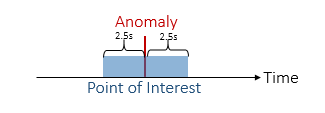
\includegraphics[width=0.75\columnwidth]{graphics/anomaly.png}
    \caption{Figure showing creation of a point of interest(blue area) from an anomaly(red line).}
    \label{[FIGURE] anomaly}
\end{figure}
To decide whether an anomaly correctly corresponds to a usability error e.g. that it \textit{hits} a usability error, some assumptions have to be made for the events.
To do so we group tasks 1, 3, 6 and 7, based on the assumption that they induce a reaction at known moments. The reasoning behind this, is that all three tasks present obtrusive visual feedback at the time of the error. Further in case of task 3, there is also audio
feedback. Task 3 displays an exception error message whenever the user attempts to open a draft, task 6 turns the
current window
black, task 7 displays a ``not responding'' window whenever the user attempts to write an email and task 1 displays an
error message after 2 seconds. Tasks 3 and 7 in particular are considered ``full stops'', and it is not possible for the
user in any way to successfully complete them. It is possible to complete tasks 1 and 6, but requires the user to
re-attempt 3 times before success. We group them equally as \textit{instant} error feedback.

Tasks 2, 4 and 5 we group as \textit{not instant}. All three tasks requires the user to notice that an error occurred, or
that the action was not successfully performed. During task 2, the user has to notice that the contact was not added,
task 4 is first noticed when the user realizes that incorrect characters appear on-screen and task 5 again requires the
user to notice that the caret has moved. While task 4 and 5 could induce an instant reaction, we cannot know for
certain that this is the case, as they might be looking at the keyboard while the error occurs and first discover it, when they look up to verify what they have written.

Given tasks' events in the experiment is grouped into ``instant error feedback'' and ``non-instant error feedback'', two strategies has to be used. 
For instant error feedback the usability error is said to have been experienced by the participant at the specific time the error happened. In other words, if the error happens at time $t$, then the participant is also exposed to the event at time $t$.
For non-instant error feedback the usability error is said to have been experienced during the timespan of the first event to the last event which are related to the task. This is illustrated in Figure \ref{[FIGURE] non-instant illustration}.
\begin{figure}
    \centering
  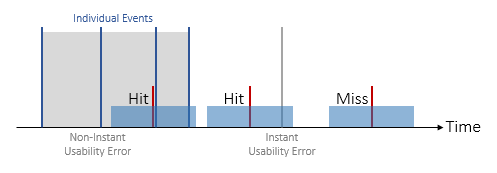
\includegraphics[width=0.75\columnwidth]{graphics/hitmiss.png}
    \caption{Each vertical blue line is an individual event, e.g. ``Caret Moved''. The combination of these make up the ``non-instant usability error''. The grey line is an ``instant usability error'', which consists only of the event it self. The points of interest(blue areas) depict a hit on a instant event an non-instant event, and also a miss.}
    \label{[FIGURE] non-instant illustration}
\end{figure}
To evaluate if an event is correctly found by the machine the two types of events are considered again.
The events which contain instant feedback is classified as a hit, if the points of interest covers the time at which the event happens.
For events which do not contain instant feedback the event will be hit, if the point of interest hits inside the area of the collection of events. Both of these examples is illustrated in Figure \ref{[FIGURE] non-instant illustration}.

Given the one-class SVM's sensitivity, a scoring function is used to optimize the gamma value in the grid search. It is defined as: 
\[CovScore = \frac{2 \times EventsHitRate \times (1-FalseCoverRate)}{EventsHitRate + (1-FalseCoverRate)}\]
Where \textit{EventHitRate}(EHR) describes how many of the existing events have been hit by an anomaly e.g.:
\[EHR = \frac{DifferentEventsHit}{TotalNumberOfEvents}\]
, and \textit{FalseCoverRate}(FCR) is the rate of which the area outside events that has been covered e.g:
\[FCR = \frac{NonEventAreaCovered}{TotalNonEventArea}\]
Machines which have a low EHR and/or high FCR would make the function approach zero, while having a high EHR and low FCR will make the function approach 1, which is the ideal result.
Meaning this function rewards hitting as many different events higher than hitting the same multiple times, while also considering the rate of FCR.

In other words the Nu value dictates the aggressiveness of the classifier, e.g how big the normal state is given its training data. A high value results in an aggressive classifier and a low values result in a conservative classifier, as illustrated in Figure~\ref{[FIGURE] nuvalues}.
Different level of aggressions will be examined to establish its impact.
This is done using a line search, keeping all the parameters constant, except the in the following range:
\[Nu = \{0.01, 0.02,.., 1\}\], and analyzing the difference in the result. 
\begin{figure}
    \centering
  \includegraphics[width=0.75\columnwidth]{graphics/nuvalues.png}
    \caption{The figure shows how the boundary changes at different Nu values}
    \label{[FIGURE] nuvalues}
\end{figure}